\chapter{Future Work}
\label{chap:6}

Potential for future work exists in a number of directions, both in the near term and long term. More pressing research opportunities and improvements to the tools discussed are outlined, followed by a discussion of grander directions in which the field of image-based modeling and simulation is moving.

%%%%%%%%%%%%%%%%%%%%%%
%%%%%%%%%%%%%%%%%%%%%%
\section{Short Term}
\label{Short Term}

Tasks related to completing the full demonstration of polyhedral FEM in Celeris, improving the image-based meshing tool Shabaka, and improving the cardiac mechanics code Cardioid are described herein.

\subsection[A Polyhedral Finite Element Demonstration in Cardiac \\ Mechanics]{\texorpdfstring{A Polyhedral Finite Element Demonstration in Cardiac Mechanics}{A Polyhedral Finite Element Demonstration in Cardiac Mechanics}}
\label{A Polyhedral Finite Element Demonstration in Cardiac Mechanics}

Pending some minor fixes in the Celeris codebase, the first task is to complete the verification problems outlined in \chapref{5}. Given the accurate results provided by Imitor, it is expected that Celeris will produce satisfactory results as well, at least for cuboidal PEM elements. The benefit of polyhedral FEM for these purposes is again three-fold: complex geometries may be meshed automatically, the mesh resolution is not constrained directly by the surface resolution, and linear element shape functions avoid an unnecessary increase in DOF. The single ventricle geometry is simple enough, though, that automated hex and tet meshing is not particularly constrained by the surface resolution in this case. Nonetheless, completing the verification problems will at a minimum show the capability to automatically generate a general polyhedral mesh and run accurate solutions while avoiding quadratic elements.

Once the implementation has been fully verified, the following step would be to run a complete bi-ventricular cardiac mechanics simulation using polyhedral finite elements. The highest priority is first to demonstrate capability, followed by a more direct comparison of results and computational effort between the quadratic tet mesh in Cardioid and the polyhedral mesh in Celeris. This would require a convergence study in both codes to ensure that the coarsest possible meshes were being used while still attaining accurate results. This likely would also include a more comprehensive comparison of results, for example by measuring and comparing stresses and strains at particular locations of interest. As of yet, there is no definitive answer to whether polyhedral FEM is a viable replacement for quadratic tetrahedra in cardiac mechanics simulations, but the preliminary results look very promising. A direct demonstration of polyhedral FEM's desirable features would be quite useful.

It is worth mentioning that for polyhedral FEM to have competitive runtimes, the associated code would likely need to incorporate an iterative solver and potentially be restructured to run on a distributed memory system. There is nothing unique to polyhedral FEM that would prohibit those changes though. Depending on the degree to which the number of DOF can be reduced, and the desired simulation resolution, a direct solver on a shared memory system may well be more than sufficient, but that would need to be proven. Additionally, the notion of \textit{element quality} has not yet been well defined in the context of polyhedral elements. Concepts related to mapping shape functions from the physical space to a parent space are obviously not an issue, but it is still unclear the degree to which elements near the boundary may be ``ill-shaped'' before solution accuracy begins to degrade. A complete bi-ventricular simulation would certainly clarify some of these matters.

Ultimately, polyhedral finite element methods would exhibit its advantages most strongly in image-based biomechanics for geometries that require a high resolution to define the surface, and for problems that require frequent remeshing during the simulation. It is hoped that these next steps would further solidify the promise of such an approach.

\subsection{Improvements to Image-Based Meshing Code}
\label{Improvements to Image-Based Meshing Code}

A vast number of improvements may be made to the image-based meshing code Shabaka, which would open several additional application areas for which the code could be useful.

The highest yield improvements involve expanding the capabilities of the interface approximation and surface reconstruction tasks. Interface approximation would be significantly improved if expanded to handle regions of high curvature or even sharp edges and corners. This would involve creating more interface ``templates'' in addition to the plane approximation that is currently in place. The most favorable additions would include a paraboloid interface, an edge interface, and a corner interface. For these interfaces, several point/normals may be placed for a single window. This extension would significantly improve the accuracy (and resulting density) of points in regions of high curvature, and even allow image-based mesh generation for objects with sharp edges and corners. The ability to generate high-quality surfaces involving sharp features would usher opportunities for more conventional mechanical and aerospace engineering applications.

Another important extension to Shabaka is handling multi-material image masks. As of now, the algorithm is restricted to binary image masks. Although plenty of work is still performed for single object meshes, the state of the art tools available for image-based meshing tend to have capability for multiple materials. Ideas may be gleaned from Dyadechko and Shashkov~\cite{dyadechko_2008}, who reconstruct polygonal multi-material interfaces for simulations of incompressible fluid flows. Although currently only developed for two dimensions, their work provides a partitioning scheme for multiple material junctions based on similar notions of minimizing error in the moments of volume. Once the matter is sorted, Shabaka may link with the same mesh generation tools as before, which are already well-equipped to handle multi-material b-reps. This improvement would significantly expand the range of biomedical applications, most notably to the brain and the knee (see \figref{polyknee}).

\begin{sidewaysfigure}[htbp!]
\centering
		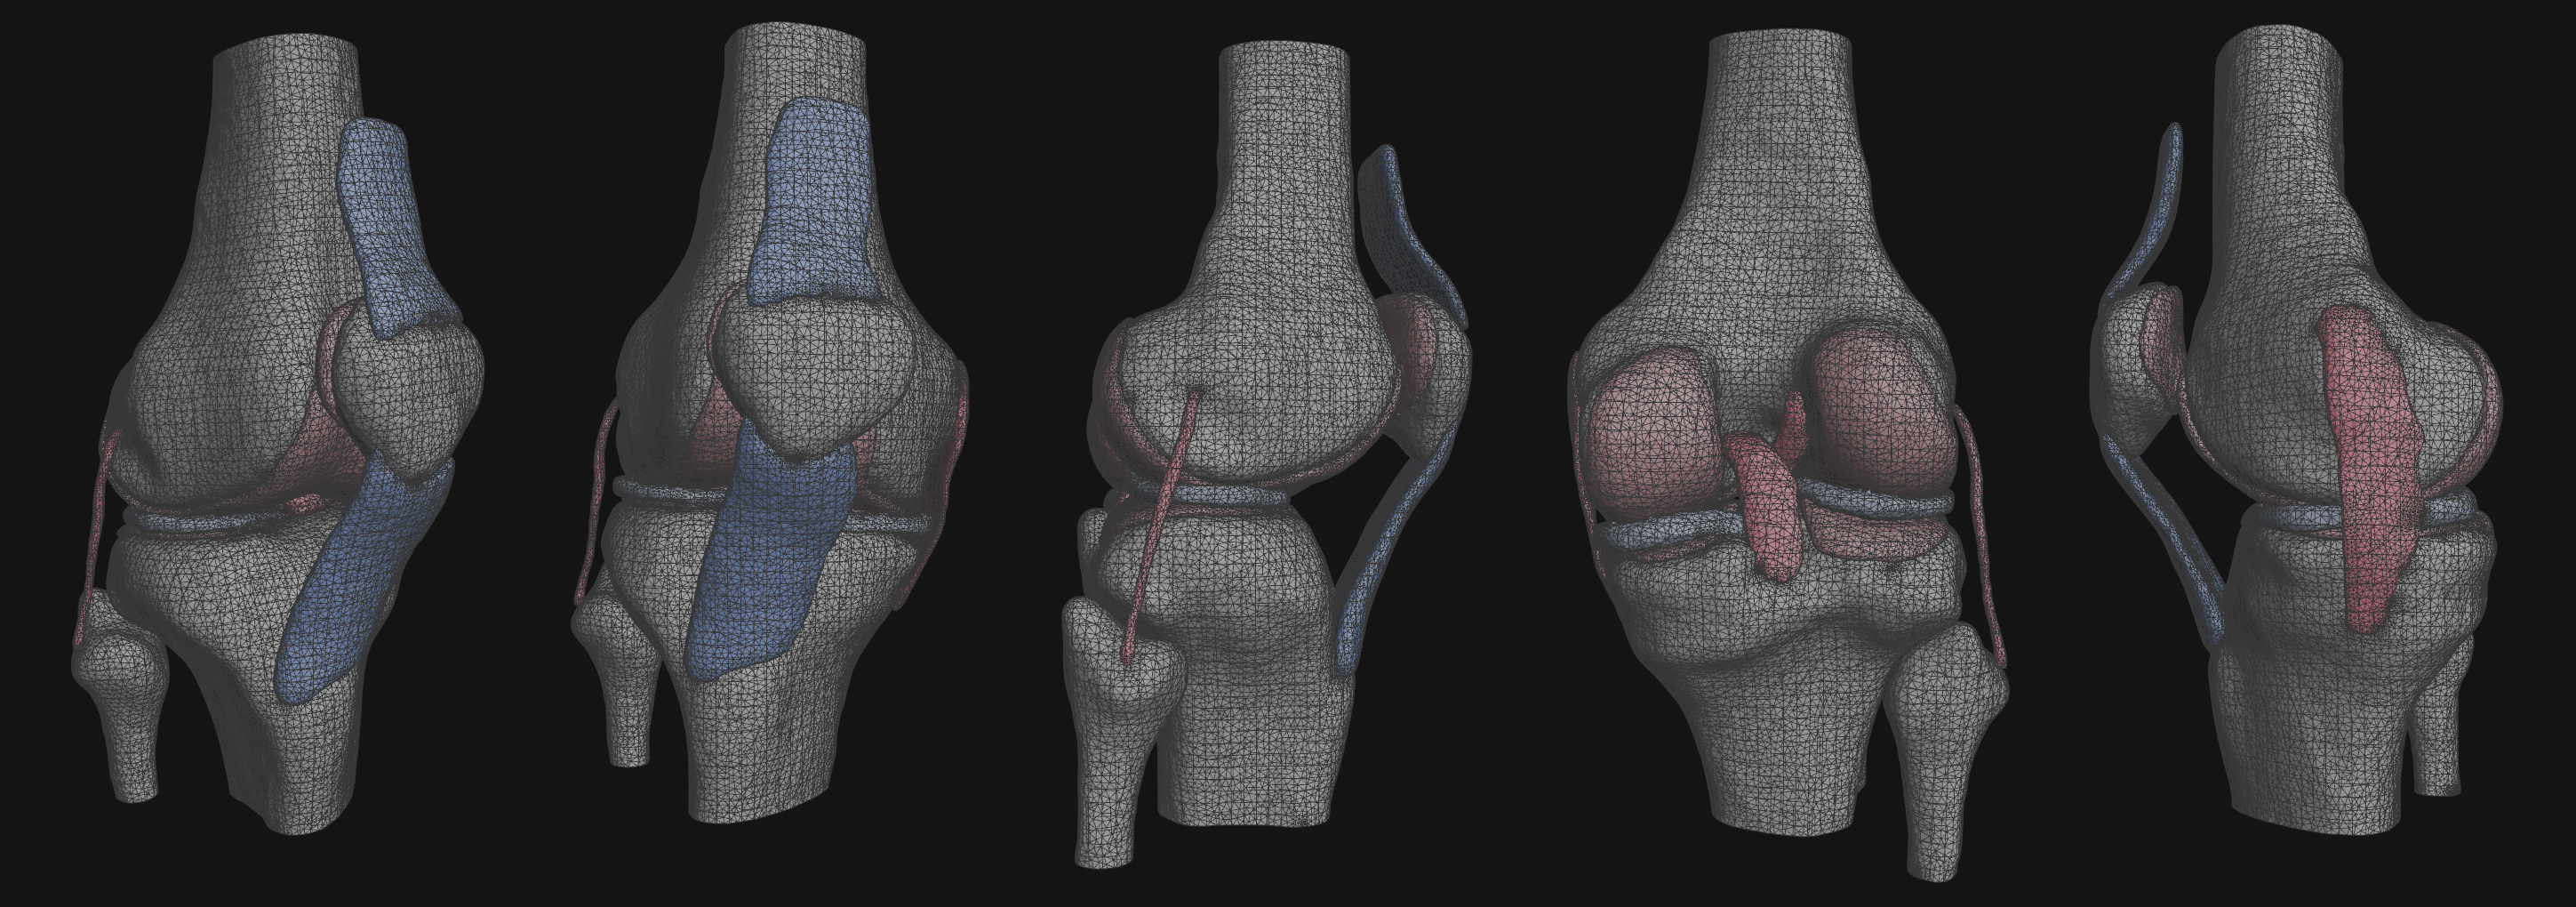
\includegraphics[width=1.0\textwidth]{media/7-polyknee/fullmesh.png}
%
\caption{Polyhedral mesh of human knee generated from Open Knee b-rep~\cite{erdemir_2015}}
\label{fig:polyknee}
\end{sidewaysfigure}

Improving the surface reconstruction of an oriented point cloud is also critical. Work is underway within the Celeris codebase to allow for a \textit{tolerance-aware} Voronoi partitioning scheme~\cite{rashid_2019}, with similar philosophy and implementation to how polyhedral meshes are constructed from b-reps. This could potentially mitigate the issue of ``cross-talk'' facets discussed in \chapref{3}. If a tolerance-aware approach does not resolve the issues caused by the current Voronoi approach, the surface reconstruction task may be better suited to follow the approach outlined by Meyer \textit{et al.}~\cite{meyer_2008}. Provided an oriented point cloud, they perform a Delaunay tetrahedralization on the point cloud itself, and then extract the surface of interest based on \textit{Delaunay} facets that share different material types.

A less urgent task would involve improving the interaction between image, image mask, and surface mesh. Work may be explored to generate point clouds directly from medical images, bypassing the image segmentation step altogether. Considering the complexity of image segmentation techniques, avoiding that intermediate step would likely prove to be a difficult task. A more fruitful intermediate term approach may be to extract more information from the image mask. For example, the underlying image carries a range of intensity values near the interface approximated by the image mask. Retaining that information with the segmented image can lead to more accurate surfaces. Indeed, Young \textit{et al.}~\cite{young_2008}, for example, make use of ``soft segmentations'', or what they call the \textit{partial volume effect} to produce smoother surfaces. In essence, they honor the fact that the image and image mask are inextricably linked.

From a software utility standpoint, the Shabaka code may be improved in some tangible ways as well. The bash build script should be replaced by a \textit{CMake}~\cite{cmake} file for a more robust installation process in downloading and installing external packages. In the same vein, the Windows version ideally would not depend on the Windows Subsystem for Linux, which is essentially a temporary workaround due to familiarity with accessing third-party software in a UNIX environment. In the interest of a faster and more reliable build, more tools should be developed within Shabaka to avoid dependence on admittedly fragile third-party software.

Finally, a necessary step in proving the quality of results from Shabaka is a numerical validation of point clouds and surface meshes for a variety of example inputs. Error measures should be defined and calculated to quantify the degree to which the interface approximations generate point clouds that honor the original surfaces from a medical image. Similarly, the quality of resulting surface meshes should be measured numerically, perhaps again comparing moments of volume between the original image mask and the resulting surface. Of course, these error measures ideally should be compared to other popular surface reconstruction and image-bashed meshing algorithms. Lastly, as coined by Young \textit{et al.}~\cite{young_2008}, the notion of \textit{convergence to geometry} must be further explored and understood. Specifically, mesh convergence from CAD data typically assumes there is no error in the geometric accuracy of the solid model itself. In image-based meshing, however, a finite number of sampling points are used to reconstruct the b-rep, and thus there is inevitably an error associated with that approximation. Shabaka does currently allow the user to specify the number of points to define the surface of interest. Further developing guidelines for how many points are actually required to ``converge to geometry'' would be quite informative and useful.

\subsection{Improvements to Cardiac Mechanics Code}
\label{Improvements to Cardiac Mechanics Code}

The cardiac mechanics code Cardioid has room for improvement on several fronts now that a robust workflow for cardiac simulations has been established. Arguably the most interesting tasks from a computing standpoint are moving towards a complete coupling between the mechanics, electrophysiology, and \textit{hemodynamics} (i.e., circulatory model) codes. As mentioned before, only a one-way coupling currently exists between the electrophysiology and mechanics codes. In reality, of course, the large deformations experienced in the heart certainly affect the manner in which electrical waves propagate within the body. Likewise, the pressures in each ventricle are certainly not spatially uniform. The current lumped circulatory model could be replaced by a complete fluid dynamics code modeling blood flow, such as the one developed by Gounley \textit{et al.}~\cite{gounley_2017}, which is also affiliated with Lawrence Livermore National Laboratory. In this case, the volume constraints would be replaced by fluid-structure interaction considerations.

Other important improvements include the treatment of boundary conditions at the base and epicardium of the heart. As of now, the less-than-convincing BCs that displacements at the base be restricted in-plane, and that an arbitrary strip of the epicardium is restrained in all three directions, must be improved. A simple improvement to the epicardium BCs, for example, could involve modeling the heart inside a fixed elastic medium. \textit{In vivo} behavior of the heart should certainly guide those decisions. Although not urgent, providing the ability to generate muscle fiber orientations directly from DTMRI data would also improve the Cardioid code. Although the process has not been perfected, some groups have been successful in moving away from model-based fiber generation~\cite{yang_2012, zhukov_2003}.

Even without the improvements suggested here, several studies may now be performed with the current model. Validation of results must be the highest priority as Cardioid moves toward answering clinical questions. Additionally, given a working model, a whole range of sensitivity studies may be performed to determine what meshing and modeling parameters are most influential. Some questions include:
\begin{itemize}[noitemsep]
\item How sensitive are the results to approximating the surface of the heart accurately? Is diligently capturing the inner structures in the ventricles necessary? Some preliminary work hints that papillary muscles, for example, do not play a significant role~\cite{korte_2019}.
\item How does the accuracy of fiber orientation affect the solution? Do fibers generated from a rule-based approach produce different results compared to those generated from DTMRI data?
\item How do different passive and active constitutive models affect the solution?
\item How does mesh quality affect the iterative solver performance?
\item To what degree do the boundary conditions influence the solution?
\item How important is it to include electromechanics coupling and/or fluid-structure interaction?
\end{itemize} 
Lastly, much in the same way convergence to geometry should be guaranteed by Shabaka, a mesh convergence study should be performed to determine the desired resolution of cardiac meshes for converged simulation results.

%%%%%%%%%%%%%%%%%%%%%%
%%%%%%%%%%%%%%%%%%%%%%
\section{Long Term}
\label{Long Term}

A brief discussion here covers the future of image-based modeling and simulation and how it might interact more with machine learning and 3D printing in the coming years.

\subsection{Simulation of Clinical Trials}
\label{Simulation of Clinical Trials}

Although plenty of opportunities still exist to improve the tools involved in image-based modeling and simulation, research in robustly performing patient-specific modeling has reached a relatively mature state. Patient-specific treatments and medical devices are already a reality. The important next step in the field is to combine simulations related to a single patient with statistical and/or machine learning technologies for large populations of patients. One may refer to this extension as \textit{simulation of clinical trials}. To properly perform such an ambitious task will involve several important considerations moving forward. Among the most important are: appropriate assignment of material properties for each patient, appropriate boundary conditions for each patient, performing rigorous verification, validation, and potentially even uncertainty quantification (VVUQ) ~\cite{NAP13395}, and heavily relying on high performance computing to perform large numbers of simulations in a timely manner.

For example, the project ``A Machine Learning System to Guide Clinical Procedures in Real-Time'' currently funded by Lawrence Livermore National Laboratory is utilizing the image-based modeling workflow that has been described, and it will certainly need to attend to many of the considerations mentioned. That project aims to improve surgical treatment of \textit{ventricular fibrillation}, the deadliest form of cardiac arrhythmia. The research aims to produce a large virtual patient dataset based on imaging data, from which machine learning tools can determine optimal locations to \textit{ablate} (or remove) portions of an arrhythmic heart. The proposed virtual population of 10-40k patients will be based on a real patient population of roughly 100. The focus of this document has been to robustly generate quality meshes for accurate simulation. With that task at a working level, the focus will shift to ensuring accurate depictions of the material behavior, boundary conditions, and overall validation of results. Provided those tasks are accomplished, machine learning-guided simulations can improve real surgeries and save real lives.

\subsection[Applications in Rapid Prototyping and Additive Manufacturing]{\texorpdfstring{Applications in Rapid Prototyping and Additive \newline Manufacturing}{Applications in Rapid Prototyping and Additive \newline Manufacturing}}
\label{Applications in Rapid Prototyping and Additive Manufacturing}

Rapid prototyping and additive manufacturing have begun to revolutionize many facets of engineering, and biomechanics applications are no exception. Indeed, in 2017 the FDA issued a guideline titled ``Technical Considerations for Additive Manufactured Medical Devices''~\cite{fda3_2016}, signifying the degree to which the technology is beginning to play an important role in medical device design.

The input requirements for a 3D printer are in fact identical to those of a CAD-based mesh generation tool: a closed, manifold surface mesh is required in both cases. STL files are by far the most popular surface mesh file format for 3D printing. Some of the STL surfaces generated using Shabaka were printed with a \textit{fused deposition modeling (FDM)} printer, in which melted material is extruded layer by layer to produce a three-dimensional object (see~\figref{3dprint}). A visual print of an object can be quite illuminating, even for a surgeon or technician who has already become accustomed to 3D computer models.

\begin{sidewaysfigure}[htbp!]
\centering
		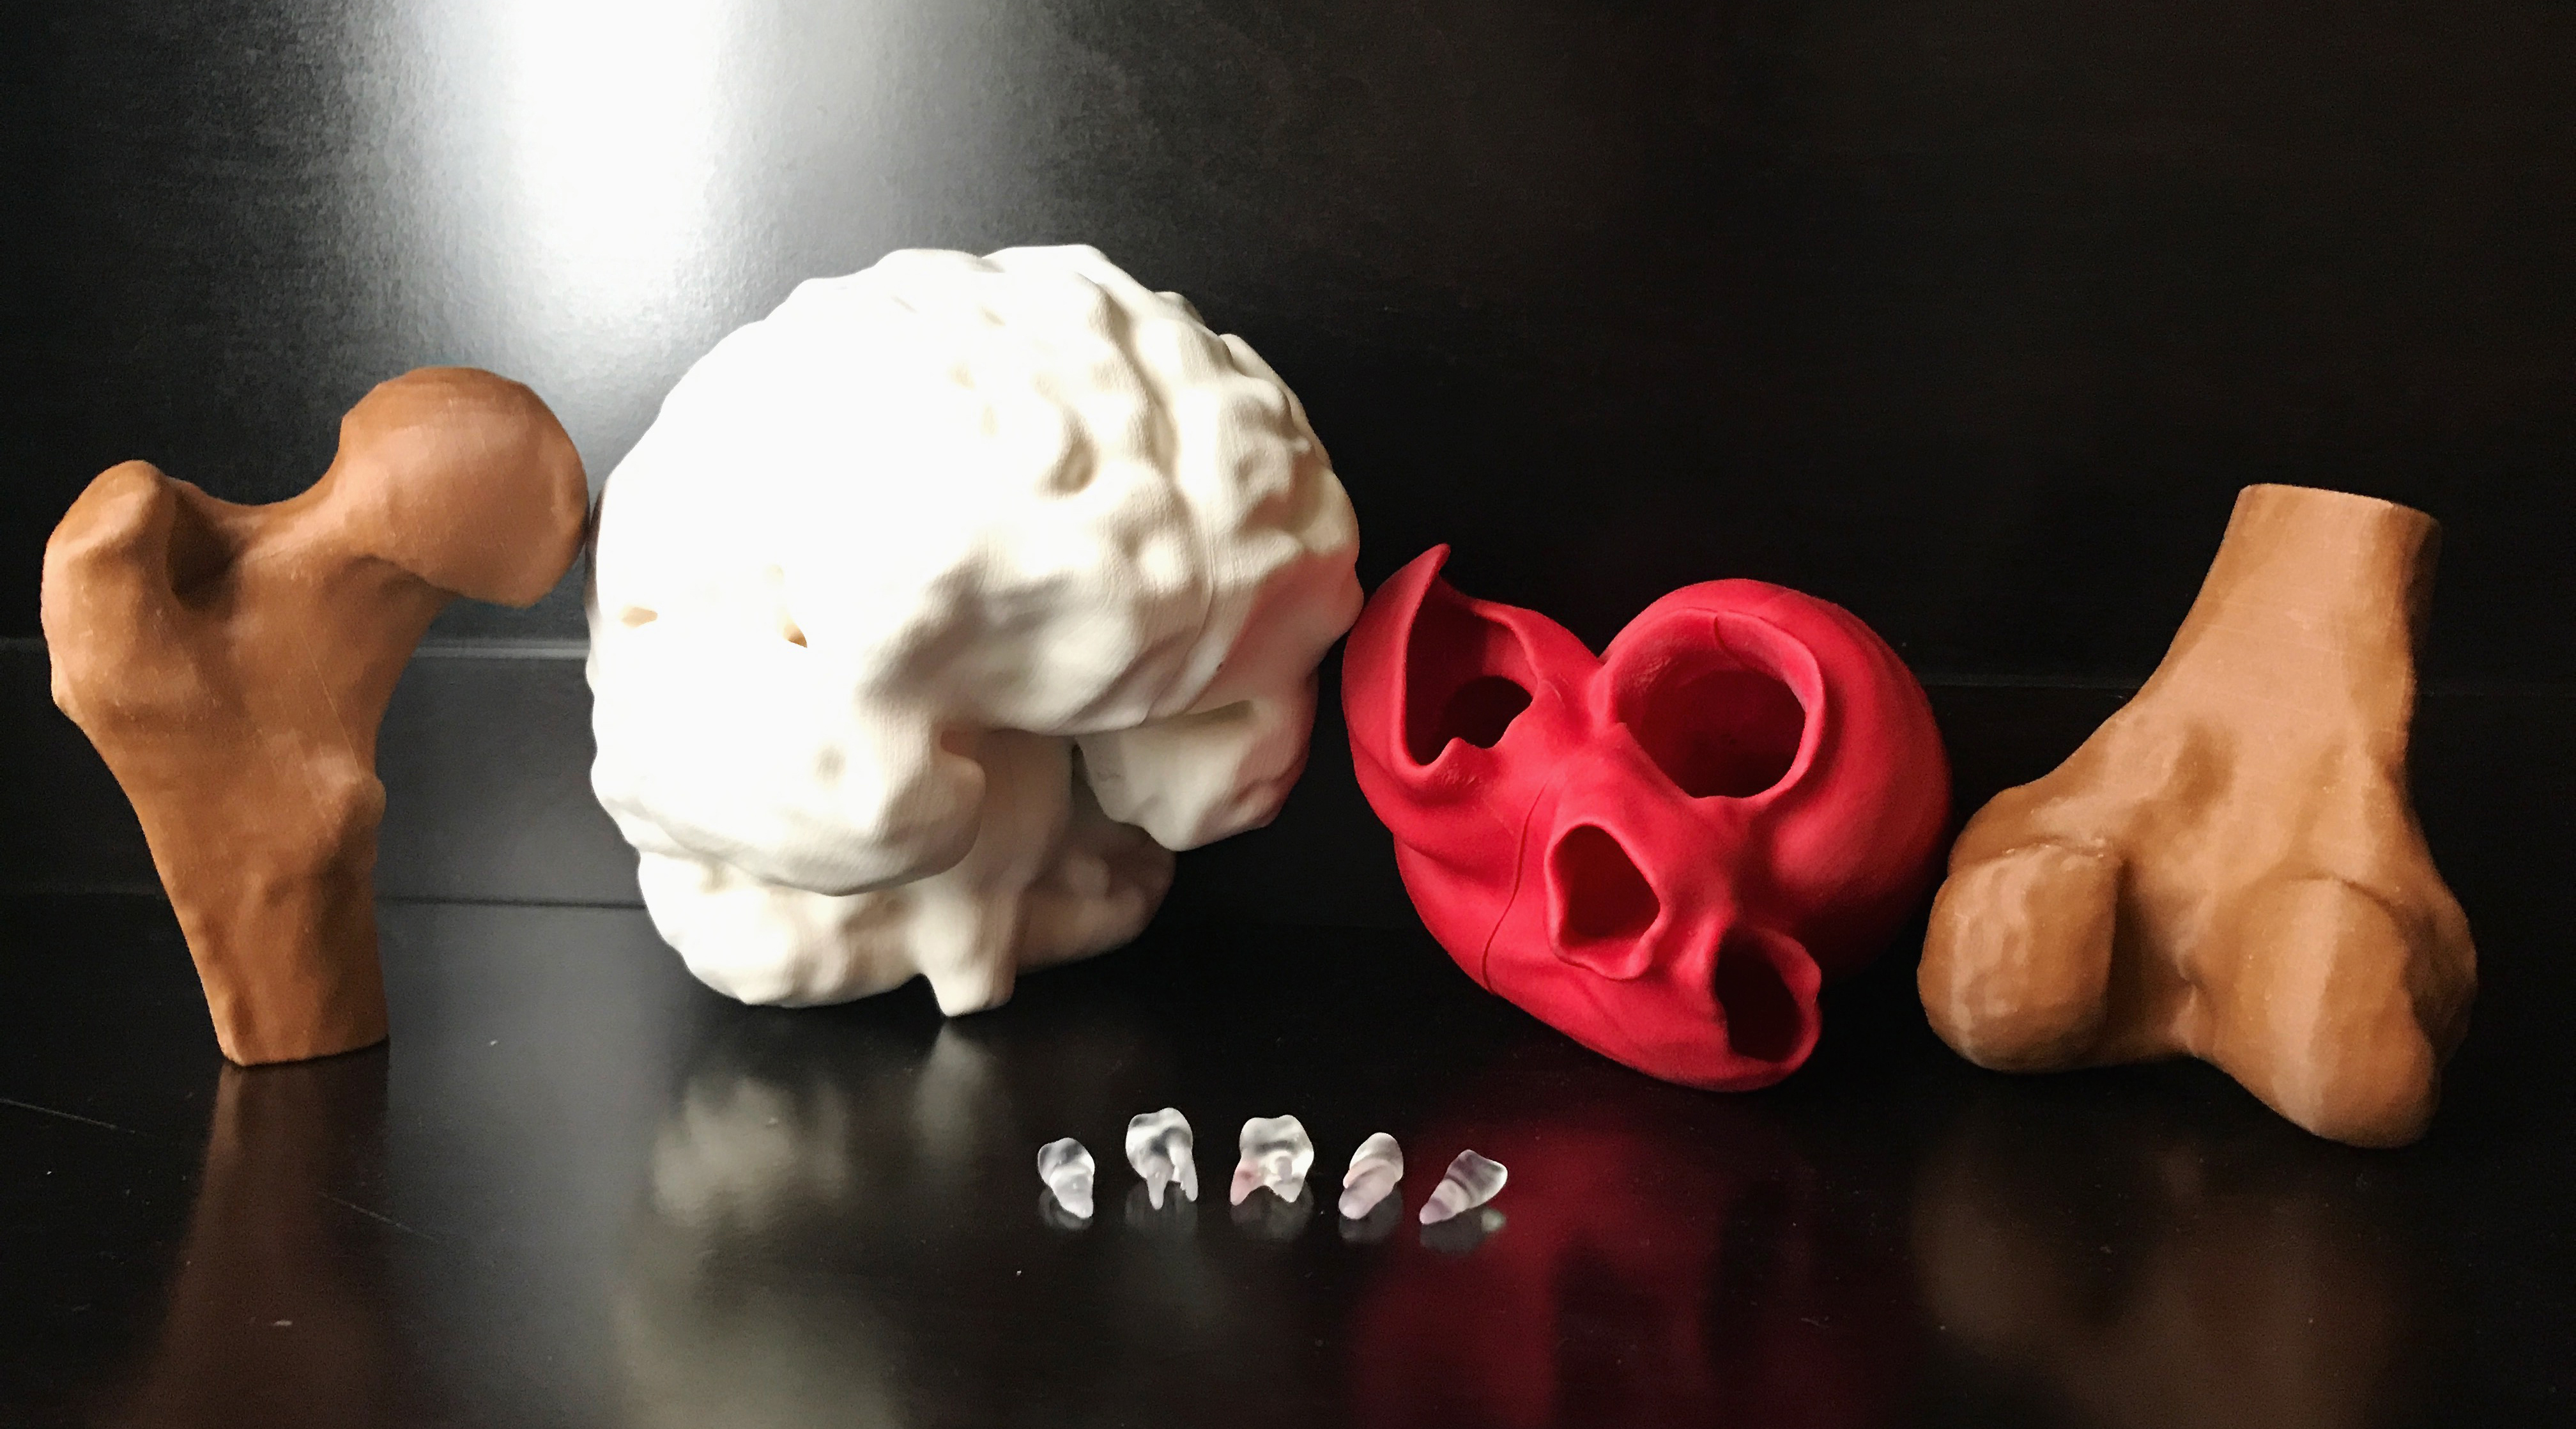
\includegraphics[width=1.0\textwidth]{media/6-3dprint/3dprint.jpg}
%
\caption{Suite of 3D-printed organs using surface meshes generated from novel image-based meshing tool Shabaka}
\label{fig:3dprint}
\end{sidewaysfigure}

Of the many challenges to robustly create 3D-printed objects using fused deposition modeling, some include:
\begin{itemize}[noitemsep]
\item reliability, i.e., getting the same output for multiple instances of the same input;
\item optimizing the many print design parameters, including extruder temperature, layer thickness, support structure, and extruder outflow rate;
\item determining the desired print precision; and
\item cost
\end{itemize}
It was deemed that fused deposition modeling is better suited for simple prototyping applications, and not for precise or large-scale applications. Other (more expensive) printing technologies will likely be more appropriate for production-level prints, such as \textit{stereolithography (SLA)}, in which a laser cures liquid resin into hardened plastic via \textit{photopolymerization}, or \textit{selective laser sintering (SLS)}, in which a high-powered laser fuses small particles of polymer or metal powder~\cite{3dprints}.

Tack \textit{et al.}~\cite{tack_2016} outlined a comprehensive review of 3D printing in medical settings. They covered various surgical domains in which 3D-printed surgical guides and implants have impacted the field, including orthopedics, cerebrovascular, cardiovascular, and dental applications. Clearly 3D printing enjoys several directions in which it could potentially improve the field of biomedical engineering, and its intimacy with simulation will certainly increase over time.
